%! TEX root = 'main.tex'
\section{Overview}
\label{sec:implant-overview}


%Critical infrastructure such as power grids comprises physical and cyber systems and assets that are vital to national security. Their failure or incapacity would have a significant impact on people's daily life on a large scale. The recent Ukrainian power grid attack, the massive blackout in south American countries~\cite{haes2019survey} demonstrated that influence not only affects people's livelihoods but even international politics. The cyberattack on the ICS system can even cause physical damage to the infrastructure~\cite{zeller2011myth}, which makes it harder to recover. Incidents such as the Stuxnet proved this point.

%Consequently, ICS has received considerable attention due to security concerns. There are many ways to breach a computer system, and most of them are focus on software-based approaches such as vulnerability hunting and exploiting, cracking of authentication and protocols. Therefore, the attacker needs to break into the network and avoid existing access control and other mitigations. Moreover, most critical infrastructures use their air-gapped network, and It may take a state-sponsored team to accomplish such as mission ~\cite{langner2011stuxnet}. 

%Under such circumstances, we believe that cyber-attacks with the assistance of physical approaches are underestimated, especially before the emergence of the so-called supply-chain attacks. Among those world-class attacks, the term APT(Advanced Persistent Threat) is often mentioned. In essence, the APT attack is an extremely well-hidden trojan that can be deployed for many years without being detected. Thus, installing the trojan and remotely triggering it is the crucial point of a successful attack.

In this paper, we present \name, an APT using a hardware implant that is used by an attacker to perform co-ordinated distributed attacks on critical infrastructure such as power grid. To achieve this, we reversed engineered a PLC and developed a prototype of hardware implant and showed that such kind of attacks can be performed even without the help of state sponsored attack groups. \name hijacks the data lines on the PLC and modifies them based on the command received by the attacker. Since the attacker can send such signals remotely, they can control various PLCs at different locations simulataneoulsy to perform an co-ordinated distributed attack on the entire power grid.

\begin{figure*}[tp!]
	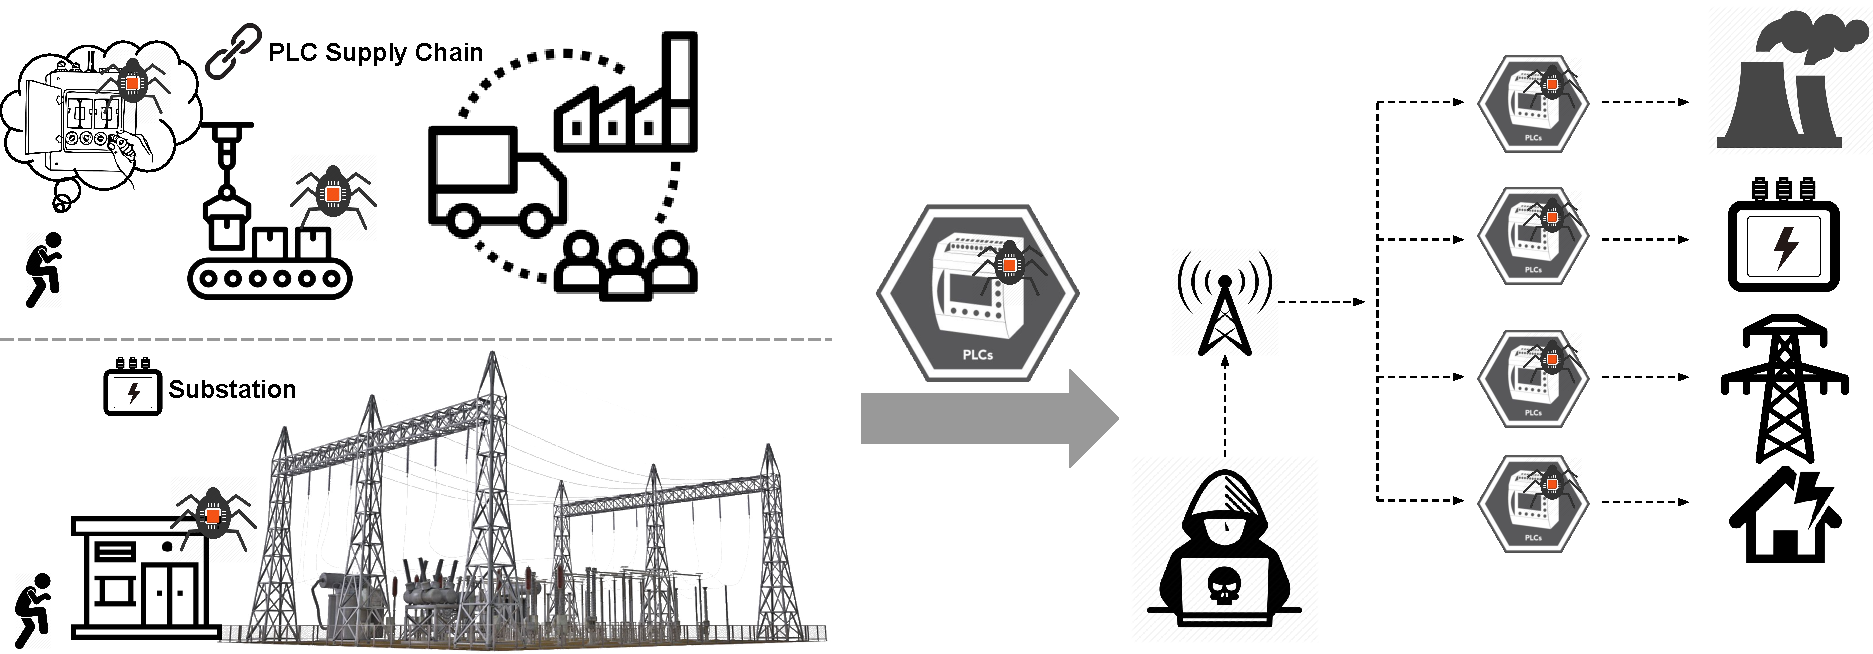
\includegraphics[width=\textwidth]{figures/bigpic}
	\centering
	\caption{In the PLC manufacturer factory or during the product shipment, numerous employees can access the PLCs. The hardware backdoor installation should follow specific procedures to be efficiently accomplished without advanced software knowledge. The hardware backdoor can communicate with the attacker through the GSM network. Therefore it does not need to join the ethernet used by the ICS system.}
	\label{fig:bigpic}
\end{figure*}

\name can be implanted into the PLC in several ways such as either installing it during the supply chain or installing the implant after the PLC is being deployed. These two scenario's are depicted in ~\autoref{fig:bigpic}. At first, during the supply chain, such as the factory and shipment, numerous employees have the opportunity to access the PLC. Installing an extra piece of a circuit board is not a difficult task for professionals~\cite{harrison2021malicious, o2015special}. Secondly, after the PLCs are being deployed, due to the vast distributed network of the power grid, it lacks strong physical security \cite{Loopholes2020}. An attacker can sneak into one of the substations and install the hardware backdoor. The difficulty between the targeted PLC and the attacker, in reality, can be just a few padlocks. We believe that the breach of a substation can cause a chain reaction in a power grid, and it is a real threat~\cite{substationattack, chen2020study}.


%In this paper, we provide two plans for physically installing a trojan and provide a prototype hardware implant \name that can be used for this type of attack. ~\autoref{fig:bigpic} depict the scenario. In many parts of the supply chain, such as the factory and shipment, numerous employees have the opportunity to access the PLC. Installing an extra piece of a circuit board is not a difficult task for professionals. Moreover, a large-scale infrastructure such as a power grid has many remote substations with very few staff. An attacker can sneak into one of the substations and install the hardware backdoor. The difficulty between the targeted PLC and the attacker, in reality, can be just a few padlocks. We believe that the breach of a substation can cause a chain reaction in a power grid, and it is a real threat~\cite{substationattack}~\cite{chen2020study}.


After the attacker controls enough PLCs, he can remotely initiate a distributed attack to cause more significant damage to the critical infrastructure using a cellular network. The advantage of this attack is that it does not rely on the existing ICS network, nor is it limited to the firmware running on PLCs so that it can evade most software-based mitigations. It only needs to know the specific PLC model of the target and modify the hardware implant accordingly.


\subsection{Adversary Model}

We assume that the attacker has physical access to the PLC once to implant the \name. Many studies and reports have shown that those are not superficial and have been done in real world~\cite{harrison2021malicious, o2015special, robertson2018big} either during manufacturing or during shipment. Since the attack is aware of the model of PLC being targeted, we assume that the attacker know the internal of the PLC. This could be assumed since the attacker can purchase an exact replica of PLC from any vendor. 

%The attacker knows the target's specific PLC model and can obtain the exact model for studying.

The printed circuit board (PCB) and the IC chips of the PLC should be well exposed. For example, the Chip-on-Board (COB)~\cite{lau1994chip} packing brings extra challenges for the attacker. The black glob-top makes it difficult to identify the chip model and pins. Fortunately, high-end microcontroller products rarely use these packaging. It would be a great advantage if the attacker can use the JTAG interface of the microcontroller. In other words, the JTAG interface is not disabled by programming fusing bits at the factory. Nevertheless, the attacker can control the IO or tamper with the firmware image when transferred through the bus without JTAG.

\name is less invasive in with regards to the firmware. Hence, there is no modifications to the operating system, the system software, or any software mitigation solutions that run on microcontroller. Hence, \name is undetected by such software mitigation solutions. The PLC system is allowed to have any memory protection mechanisms based on MMU~\cite{shalan2000dynamic} and MPU~\cite{kim2018securing}.

To remotely control the device, the attacker uses a GSM network or WIFI to communicate with the hardware backdoor. The PLC must not be deployed in an electromagnetic isolation environment (Faraday cage) where the wireless signal can not be transmitted outside. This is reasonable assumptions since lot of communications in such substations happen through wireless communications used by remote terminal units (RTUs).



\subsection{Challenges}

The major challenge in attacking PLCs is not having enough information about the device. Some vendors publish the microcontroller's datasheet, but some vendors use proprietary design with highly customized instruction set architecture (ISA).  The layout of the PCB board and the on-board pin definition are also not publicly available.


\textbf{\textit{Firmware.}} In an embedded system, flash memory usually stores a file system and a real-time operating system (RTOS) such as VxWorks~\cite{neugass1991vxworks}. It is the so-called firmware. Specific to a real-time microcontroller, the firmware runs bare-metally on the microcontroller or with a lightweight RTOS such as FreeRTOS~\cite{barry2008freertos}. Allen Bradley 1769-L18ER-BBIB CompactLogix 5370 has very limited information about the firmware being used. 

\textbf{\textit{Identifying Components on Board.}} Due to the lack of information and lot of proprietary chips used by such vendors, it is difficult to identify the chips used on the PLC board. Some of the chips have BGA packaging~\cite{joshi2000mosfet} where the pins are buried underneath. So it is difficult to trace the circuit board and identify the connections and pins such as JTAG. 

\textbf{\textit{Prototype.}} The main challenge of developing such an implant is the power consumption of such an implant. To reduce the footprint, a small chip had to be used, that contains all the tools that could be used for hijacking, information retrieval and modification of the signals. Not many tools are present for such a bare metal implants and they have to be ported to work on minimal computing base.   
